\documentclass{article}
\usepackage[margin=1.5in]{geometry}
\usepackage[utf8]{inputenc}
\usepackage{graphicx}
\usepackage{hyperref}



\title{
    \Large Replication of "Clearing the Air? The Effects of Gasoline Content
Regulation on Air Quality" by Auffhammer and Kellogg (2011)\footnote{Final Project for STAT 156 taught by Professor Peng Ding during Fall 2021}}
\author{Danny Wu}
\date{December 15, 2021}


\begin{document}

\maketitle

\section{Introduction}

With the passage of the Clean Air Act in 1963, US federal and state governments became committed to the reduction of ground-level ozone. Ozone, a colorless odorless gas connected to various health risks, is produced by the reaction of volatile organic compounds (VOCs), and nitrogen oxides (NOx), both of which used to be common industrial pollutants. The main regulatory strategy employed to limit ground-level ozone is thus to limit the emission of VOCs and NOx. Many state and federal regulations target gasoline content, as highly reactive VOCs such as benzene, butane, and toluene are common gasoline additives. Gasoline content regulations are problematic, however, as regulatory differences can disrupt interstate gasoline markets, creating unnatural economic pressure on gas prices. Thus, in “Cleaning the Air? The Effects of Gasoline Content Regulation on Air Quality,” Maximillian Auffhammer and Ryan Kellogg analyzed the efficacy of gasoline content regulations in decreasing ground-level ozone in order to assess the economic value of gasoline content regulations. This paper is a replication of Auffhammer \& Kellogg’s analysis. According to Auffhammer \& Kellogg, California’s “Reid Vapor Pressure Regulations” were the only gasoline content regulations that were successful in reducing ground-level ozone, as federal gasoline content regulations aimed at reducing VOC emissions failed to have any substantial effect on ground-level ozone. This failure is attributed to the federal regulation’s flexibility, as refiners were allowed to choose which VOCs to remove from their product, resulting in the removal of less reactive VOCs. In contrast, California’s regulations targeted specific VOCs (butane), which contribute the most to ground-level ozone. 

\section{Data and Cleaning}


The data used is the EPA’s Air Quality Monitor data from 1989 to 2003. This data provides hourly observation of various air quality measurements. For our purposes, we will be specifically looking at ozone level measurements. Using this data, measures of the daily maximum concentration and daily eight hour maximum were constructed. The relevant data was cleaned in four ways: first, monitor-days in which observations were not recorded for at least 9 hours were removed. Second, monitor-years for which 25\% of monitor days during Summer report no observation were removed. Third, data from counties neighboring countries with stricter regulations was removed. Finally, all non-US (Canadian) data was removed. In total, 1,160,372 observations were included in the data set, with 728 unique air quality monitor locations in 1989, and monitor-days increasing by ~2\% every year. This data was then combined with weather observations from the National Climatic Data Center’s Cooperative Station Data (NOAA 2008). Ozone monitoring stations were matched with the 10 closest weather stations based on the euclidean distance as calculated by their longitude and latitude coordinates. Then, a primary weather station was chosen based on which weather station had the most matching observation times with the ozone station. 

\section{Summary Statistics}

We produce a summary statistics table and a graph from the cleaned data. Table  \ref{tab:summaryStats} contains the number of total observations per year, and how many of the total observations each year were from monitoring stations in rural, urban, and suburban areas. The graph shows the fluctuations of ozone levels according to gasoline regulation. The summary statistics table produced by our data is practically the same as Auffhammer and Kellogg’s. There is a slight difference in the number of monitoring stations observed in our data, however our data has more observations after being cleaned than theirs. As we followed the same steps as Auffhammer and Kellogg in our data cleaning process, we decide this is due to differences in our base data set, as the EPA mentions retroactively adding observational data. Hence, we keep the extra observations as it more accurately reflectly the real world.  


\section{Method}

Our goal in this paper is to replicate the observed effects of gasoline content regulations on ambient ozone concentrations from “Cleaning the Air” by Maximillian Auffhammer and Ryan Kellogg. To that end, various regulatory frameworks were considered. 

The authors first analyze the Reid Vapor Pressure (RVP) regulations which were initially enacted in 1989 with varying limits across different states corresponding to the level of emission reductions that were needed. More lenient states had a lower standard of 10.5 or 9.5 psi while most states had tighet requirements of 9.0 psi. In 1992, the second phase of RVP began, which required all counties to meet the 9.0 psi limit, with some states being mandated an even more strict 7.8 psi limit due to their level of emissions. 

Next, in 1995, the EPA began to enforce the Clean Air Act Amendments of 1990, which consisted of reformulated gasoline regulations (RFG). RFG was mandated for severe areas with high levels of pollution, however less polluted areas had the option to opt-in to federal RFG as a way to decrease their emissions in an effort to reach the EPA's desired attainment levles. RFG regulations are similar to RVP, however are tighter and involve more constraints on what are acceptable emissions. 

Lastly, in March 1996, the California Air Resources Board (CARB) gasoline was required throughout all of California, and target emissions even more stringently than RFG and RVP. By using heterogeneity in policy enactment across the United States as well as the variation in the severity of regulation over time, the authors were able to ascertain the effectiveness of different types of gasoline content regulations on reducing ambient ozone levels.

Auffhammer and Kellogg determined the efficacy of each regulatory framework through Difference-in-Differences (DD) as well as Regression Discontinuity (RD) analysis. For the purposes of this replication, only the Difference-in-Differences analysis is considered due to bandwidth limitations (see section 6). 

\section{Empirical Strategy}

Auffhammer and Kellogg first attempted to identify the causal effect of these different waves of gasoline regulations using a difference-in-differences (DD) method. In their approach, they compare the change in air quality following the introduction of a specific regulation (hereafter refered to as treatment) to contemporaneous change in areas that did not receive that same treatment. As mentioned previously, RVP Phase II, RFG, and CARB were only implemented in certain areas and were all implemented at different times. Most counties can be considered control, as they have had the same RVP regulation with a 9.0 psi limit since 1989. 

\subsection{Difference-In-Difference Model 1}
The first and most basic DD model has the following functional form, with $i$ indexing for individual ozone monitors, $t$ indexing for the two measures of ozone (daily maximum level and daily 8 hour maximum), $c$ indexing for the four different treatments (RVPI, RVPII, RFG, CARB), and $r$ and $y$ indexing for census region and year: 

$$\ln{(y_{it})} = \alpha \cdot \textbf{Treat}_{ct} + \mu_i + \eta_{ry} + \epsilon_{it}$$ 

$\mu_i$ and $\eta_{ry}$ are fixed effects for each individual monitor and the interaction between census region and year. These account for general differences in ozone levels at each monitor and unobserved year to year shocks in each census region respectively. 

For this model, the authors assume that "county-specific unobserved factors affecting ozone concentrations are constant over time" (Auffhammer \& Kellogg, p.  2699). This is integral to their difference-in-differences methodology and identifying the causal effect of the policies, as they must assume that if the policies had not been enacted, the potential outcome of each county's ozone levels would have followed the same trend-line. In other words, the authors assume that unobserved factors would not cause ozone concentrations to decrease over time. They also formally assume ignorability, expressed as: 

$$E[\textbf{Treat}_{ct} \cdot \epsilon_{it} | \mu_i , \eta_{ry}] = 0$$ 


\subsection{Difference-In-Difference Model 2}

The author's second DD model includes more covariates to control for more factors that can potentially affect the ozone levels. Specifically, they bring in National Oceanic and Atmospheric Administration (NOAA) weather data readings from the closest weather station for each ozone monitor location and control for interactions between weather and time. They update the initial DD model as follows: 
$$\ln{(y_{it})} = \alpha \cdot \textbf{Treat}_{ct} + \beta \cdot \textbf{W}_{it} + \gamma_r \cdot \textbf{D}_t + \delta \cdot \textbf{I}_{ct} $$
$$+  \theta \cdot \textbf{Trend}_{rct} + \mu_i + \eta_{ry} + \epsilon_{it}$$

$\textbf{W}_{it}$ refers to a complex sum of quadratic and cubic weather terms to control for various weather patterns over time as well as interactions between weather and \textit{day-of-week} and \textit{day-of-year} fixed effects. $\textbf{D}_t$ represents the \textit{day-of-week} and \textit{day-of-year} fixed effects by themselves. Lastly, $\textbf{Trend}_{rct}$ represents linear time trends that are specific to each county within each census region. For this model, the only assumption they make is ignorability, that is, the "unobserved factors are not correlated with treatment, conditional on the covariates"  (Auffhammer \& Kellogg, p.  2700). In mathematical terms: 

$$E[\textbf{Treat}_{ct} \cdot \epsilon_{it} | \textbf{W}_{it}, \textbf{D}_{t}, \textbf{I}_{ct}, \textbf{Trend}_{rct}, \mu_i , \eta_{ry}] = 0$$ 

They acknowledge that this assumption might be invalid if there are any other unobserved factors that affect ozone in a way that is not captured by the covariates. 

\subsection{Regression Discontinuity Model}
After the difference-in-difference analysis, Auffhammer and Kellogg attempted to identify causal effect of the different waves of gasoline regulations using a regression discontinuity model. In this approach, they measure the immediate effect that the implementation of a regulation has on ambient ozone concentrations. Thus, when compared to the Difference-In-Difference model, Auffhammer and Kellogg's linear discontinuity model focuses on a significantly shorter time period. As a result, a more lenient identification assumption is proposed: "the RD assumption permits unobserved to act nonlinearly over time, so long as they are not discontinuous when gasoline regulations pass" (Auffhammer \& Kellogg, p.  2701). The regression discontinuity model is given as follows: 

$$\ln{(y_{it})} = \alpha_i \cdot \textbf{Treat}_{ct} + \beta_{i} \cdot \textbf{W}_{it} + f_{i}(Date_t) + \mu_i  + \epsilon_{it}$$


$\textbf{W}_{it}$ again refers to a complex sum of quadratic and cubic weather terms. $\textbf{D}_{t}$ from the second DD model is here replaced with $f_{i}(Date_t)$, an eighth-order Chebychev polynomial in time that is monitor specific. Both $\beta_{i}$, the weather correction variable, and the treatment effect $\alpha_{i}$ are monitor specific. 

\section{Replication}

As stated above, the authors' DD models include fixed effects for each individual monitor as well as multiple terms interacted with each other. This, combined with the fact that we have roughly 1.14 million observations results in a roughly $1.14 \times 10^6$ by 1600 matrix of observations and features even for the most basic difference in difference regression. This was only further exacerbated by additional features in the regression discontinuity model. Simply put, as college students, our laptops do not have the computational power to run OLS regressions with such a large number of features. Therefore, we had to make some simplifications to our DD analysis in order to reproduce their results, and the regression discontinuity analysis is not reproduced here. 

In the first DD model, rather than adding fixed effects for each individual monitor, we included fixed effects for each state, and keep all of the other variables. This decreases the size of the matrix to just $1.14 \times 10^6$ by 140, which is within the computation limits of our machines. The results are presented in Table \ref{tab:DD1regression1} and \ref{tab:DD1regression2} in the appendix. Shown are the regression of the four treatments with the dependent variable being the log of the daily maximum level of ozone, and the second being the treatments for the log of the daily 8 hour maximum ozone. Overall, our results, though slightly different from the authors', confirm their findings. Neither RVPI nor RVPII had any significant impact on ozone, while CARB standards have been shown to have a large effect on ambient ozone concentrations: we estimate that CARB standards decreased ozone concentrations by 7.78 percent. RFG regulations appeared to have a moderate effect on ozone concentrations. We thus conclude, like Auffhammer and Kellogg, that CARB standards are more effective than RVPI, RVPII, and Federal RFG standards.   
 
Clearly, since the second DD model is an extension of the first, it would be impossible to reproduce without simplification. To be able to run the regression, we once again simplify the fixed effects to only include each state rather than each of the 1,500 unique monitors. While we include all of the weather covariates, we remove the interaction between the weather covariates and the day of year variables as that consists of an additional 1200 columns in our matrix. Lastly, we stratify by whether monitors are classified as urban, suburban, or rural. This allows us to run a regression on only a subset of the data, allowing it to be less resource intensive. Our findings are summarized in Table \ref{tab:stratifiedDD2} in the appendix and are similar to the results obtained by the authors. By and large, the findings reaffirm that CARB is the most effective policy of the four treatments. While data for the CARB standards had little variation across strata, federal RFG and RVI were inconsistent. In fact, stratifying by urban designation highlights the fact that RVPI and RVPII tended to increase ozone levels relative of the baseline of 9.0 psi. CARB and RVPI standards were the most effective in suburban areas, and the least effective in rural areas.

\section{Critique}

Given the nature of Auffhammer and Kellogg's study, the use of fixed effects is understandable, as the number of unobserved variables should be a serious worry. At the same time, however, it is our view that Auffhammer and Kellogg's use of fixed effects was excessive. Aufhammer and Kellogg included intercept terms for every day of the year, every day of the week, every monitor region, every census region, every census region interacted with year, etc. This over reliance on indicators for capturing uncontrolled variables for each of the monitors and variables, in our view, likely led to overfitting. Thus, one might question Auffhammer and Kellogg's exact results due to the over-use of fixed effects. Such a critique, however, would not be enough to overturn the ultimate conclusion of the analysis, as CARB standards remain consistently effective in reducing ambient ozone concentrations. 


With regard to the DD and regression discontinuity analyses, Auffhammer and Kellogg do not properly justify the identification assumptions necessary for each analysis. The assumption that unobservable factors affecting ozone levels would remain constant without treatment requires some justification, as ozone levels tend to wildly fluctuate. Auffhammer and Kellogg provide no such justification. This is problematic, as if it cannot be assumed that ozone levels would remain constant without treatment, DD and regression discontinuity analysis is impossible. In Auffhammer and Kellogg's place, one might make an argument that such an assumption was justified. One might argue: since social attitudes towards climate and environmental issues during this era were generally constant, general awareness about environmental issues might hold emissions relatively constant. Without such an argument, however, Auffhammer and Kellogg's assumption would appear unreasonable, as ozone levels tend fluctuate unpredictably.

\section{Robustness}

 In "Clearing the Air?" rather than robustness checks, Auffhammer and Kellogg present a causal explanation for their results, arguing that reduced butane emissions both explain and prove their results. As a result, we performed a number of robustness checks in order to confirm the main results robustness. This paper will thus contain both a reconstruction of Auffhammer and Kellog's argument, as well as original robustness checks.

\subsection{Butane and Ozone Concentrations}

After their causal analysis, Auffhammer and Kellogg argue that the failure of RVP and RFG regulations to reduce ozone concentrations was due to their flexibility. In order to be compliant with RVP and RFG regulations, refiners were required to limit the total volume of volatile organic compounds (VOCs) that they emitted. In comparison to CARB standards, RVP and RFG regulations are considered "flexible," as they allowed refiners to choose which VOCs they limit, while CARB standards require the limitation of specific VOCs. This flexibility proved problematic, as the cheapest VOCs to remove from gasoline happened to contribute the least to ozone production. This problem with RVP and RFG regulations was exemplified by Butane. Butane, though inexpensive to remove from gasoline, does not significantly contribute to ozone concentrations. Thus, Auffhammer and Kellogg argue, though RVP and RFG standards reduced the total volume of VOCs in gasoline, this reduction did not translate into reductions in ambient ozone concentrations. Auffhammer and Kellogg justify this point through observations of butane emissions. Auffhammer and Kellogg provide evidence showing that after the implementation of RVP and RFG regulations, refiners began producing exponentially more butane as waste, and net emissions of butane fell while similar VOCs like pentane and hexane saw increased emissions. Auffhammer and Kellogg thus take this as evidence that their analysis is correct, as it accurately describes the expected outcome of RVP and RFG regulations, given their limits were met by the removal of butane (Auffhammer \& Kellogg, p.  2717). 

\subsection{Original Robustness Checks}

In "Clearing the Air?" Maximilian Auffhammer and Ryan Kellogg did not explicitly perform any robustness checks. This was a mistake. Multiple aspects of the given model were questionable, which could make the main result relatively fragile. Thus, we performed two original robustness checks in order to verify the robustness of the main result. For our first robustness check, we made the data more coarse, by focusing on fixed effects at the state level instead of the monitor level. For second robustness check, we demeaned all of the observations, in order to test Auffhammer and Kellogg's use of fixed effects.

\subsection{Coarse-Grained Analysis}

For our first robustness check, we made our data coarser, in order to test whether the analysis would hold for less specific models. In the original analysis, each individual ozone monitor had its own intercept. Thus, instead of considering fixed effects for each monitor, we instead considered having intercepts for groups of monitors. Specifically, we grouped monitors by state. Each state was given its own intercept term, which might be thought of as one-hot encoding the state of each ozone monitor. This approach is coarser than the original analysis, as rather than removing specific differences in ozone measurement on a monitor level, differences between monitors were leveled on a state level. In other words, rather than subtracting variation on the monitor level, we did so at the state level.

\subsubsection{Results}

In the original analysis, Auffhammer and Kellogg reported both max ozone concentrations as well as "8-hour-max" ozone concentrations. Thus, for this analysis, both statistics were reported. These results for the coarse-grained analysis are reported in Tables \ref{tab:DD1regression1} and \ref{tab:DD1regression2}  in the appendix section of this submission. With regard to the simple coarse-grained analysis, while there was some variation in the coefficients, the differences were ultimately insignificant. Variation in the data appears to follow no pattern, thus, grouping monitors by state appears to have little effect on the analysis. Just as before, RVP regulations had no marked effect on ambient ozone regulations. Conversely, RFG and CARB standards resulted in significant reductions in ozone concentrations, though CARB standards far out-performed RFG regulations. 
 

\subsection{Demeaned Analysis}

In Aufhammer and Kellogg's original analysis, there was an excessive use of fixed effects. Fixed effects for each monitor were interpreted as an intercept term for each of the roughly 1,500 unique ozone monitors over the entire time period. This approach added roughly an extra 1,500 features to the design matrix which complicated OLS procedures as such an analysis requires a large amount of computing resources. Further, the overuse of fixed effects might result in over fitting. Thus, we executed a demeaned analysis as a robustness check in order to solve this issue. To that end, we demeaned each of the ozone monitors' measurements, incorporating an intercept term for each monitor. To do this, we collected all observed measurements for each monitor, calculated the average, then subtracted this value from the measurements of each monitor. Next, using these demeaned measurements as the outcome, we ran a number of analyses of varying complexity.

\subsubsection{Results}

In the original analysis, Auffhammer and Kellogg used two separate difference in differences (DD) analyses in order to determine the efficacy of each regulatory framework. Thus, for this robustness check, we performed two separate demeaned analyses; one for Auffhammer and Kellogg's simple DD model, and another for their complex DD model. Results for the simple demeaned analysis are reported in Tables \ref{tab:robust_table1} and \ref{tab:robust_table2} in the appendix. With regard to the simple DD model, though the results from the demeaned analysis are different, they nonetheless lead to the same conclusions about each regulatory framework. RVP and RFG regulations had mediocre to negative impacts on ozone concentrations, while CARB regulations resulted in by far the most reduction in ambient ozone concentrations. With regard to the complex DD model, we performed multiple analysis of various complexity, and our results are reported in Table \ref{tab:robust_table2} in the appendix section. While the results obtained from the demeaned complex DD analysis fits with the original analysis, there were some glaring discrepancies. First, the coefficient for RVP I was significantly higher in the first and second models when compared to the original, suggesting RVP regulations lead to increases in ambient ozone. Further, the coefficient for CARB regulations generally became smaller, contesting the stated effectiveness CARB regulations from the original analysis. Despite these results, however, the ultimate conclusion of each analysis matches the main analysis. While RVP and RFG regulations did little to positively effect ambient ozone concentrations, CARB standards led to significant decreases in ozone concentrations (even if those decreases are lower than was originally reported). From this, the main result appears robust. While Auffhammer and Kellogg's data appears relatively sensitive to changes in the relevant fixed effects, their conclusions do not. 


\subsection{Conclusion}

Following these robustness checks, it is clear that Auffhammer and Kellogg's use of fixed effects had a marked impact on their results. This is exemplified by the wild variation between complex models in our demeaned analysis. These results, however, go no further than challenging the relative effectiveness of each regulatory framework. For (nearly) all analyses, CARB standards far outperformed both RFG and RVP regulations. Further, according to every model, CARB standards resulted in a decrease in ambient ozone concentrations. Thus, it is our view that both robustness checks were successful. With regard to the coarse-grained analysis, making the data coarser had little effect on the resulting coefficients. Thus, Auffhammer and Kellogg's analysis is not sensitive to generalization on the state-level. Auffhammer and Kellogg's results thus appear generally robust as they might accurately extrapolate the effectiveness of state-wide gasoline content regulations from individual monitor data. Moving to the demeaned analysis, Auffhammer and Kellogg's analysis appears somewhat inconsistent. With regard to the simple analysis, though the results for RVP and RFG regulations are similar to the original analysis, CARB standards appear much less effective. Further, with regard to the complex analyses, the coefficient for CARB standards dropped as low as 0.00, while coefficients for RVPI ranged from 0.05 to 0.01. These variations suggest that the complex DD model is relatively sensitive, as removing various features resulted in wildly different results. It is our view, however, that these results do not dissuade the relevant conclusions of "Clearing the Air?" While the results of our demeaned robustness check might suggest that CARB standards were not as effective as first suggested, CARB standards were nonetheless the most effective regulatory framework in all but one model. Similarly, while one might conclude that RVP regulations resulted in increased ambient ozone levels, such a result does not contradict the original conclusion that RVP regulations were totally ineffective in curtailing ambient ozone concentrations. Thus, while Auffhammer and Kellogg's analysis appears relatively sensitive to the removal of various features, their conclusions nonetheless hold for each model. Thus, it is our view that the replicated results are robust.


\section{Reanalysis}

Having replicated Auffhammer and Kellogg's results in "Clearing the Air," we now turn to an original reanalysis of the relevant data. From the above replication of "Clearing the Air," we determined two main goals for the following reanalysis of the data: First, we want to avoid Auffhammer and Kellogg's excessive use of fixed effects. Second, we want to use a method directly comparable to the methods Kellogg and Auffhammer used in "Cleaning the Air," so that we might easily compare our results. As a result of these goals, we chose a difference-in-means analysis for our reanalysis. It is our view that a difference-in-means analysis alone would both meet our goals and satisfy time constraints. Further topics from the course that we might have used in our analysis suffer from computation issues (regression discontinuity), redundancy (Difference in Differences), or fell short of a full analysis. Thus, for the purposes of this reanalysis, we use difference-in-means analysis in order to determine the effect of gasoline content regulations on ambient ozone content.

\subsection {Empirical Strategy}
In "Clearing the Air," Auffhammer and Kellogg determined the efficacy of each regulatory framework through Difference-in-Differences(DD) analysis. As a result, Kellogg and Auffhammer make an explicit assumption: ”county-specific unobserved factors affecting ozone concentrations are constant over time” (Auffhammer \& Kellogg, p. 2699). Such an assumption is necessary for DD analysis, as if unobserved factors caused ozone concentrations to decrease over time, such effects would be indistinguishable from the effects of CARB, RVP, or RFG regulations. A difference-in-means analysis was chosen, in part, as a result of this assumption. Similar to DD analysis, difference-in-means relies upon the assumption that ozone concentrations would remain constant without treatment (the introduction of regulations). Further reasons for the selection of a difference-in-means analysis relate to Auffhammer and Kellogg's use of regression discontinuity. As a result of computational constraints, we were unable to replicate Auffhammer and Kellogg's regression discontinuity analysis in our initial replication. Auffhammer and Kellogg's use of regression discontinuity remains impractical for this reanalysis. Nonetheless, in using a difference-in-means analysis, we might gain insight as to what the results of a regression discontinuity analysis would be. Limiting our analysis to the period immediately following the introduction of gasoline regulations gives a picture as to the immediate effect of those regulations. Thus, we might extrapolate the results of a regression discontinuity analysis from a difference-in-means analysis. A difference-in-means analysis also meets both of our initial goals for this reanalysis. With relation to our first goal of avoiding fixed effects, a difference-in-means analysis allows us to provide analysis without any of the fixed effects used by Auffhammer and Kellogg. Instead of directly incorporating fixed effects and covariates, we graphed  covariates along with our results to show how they might have influenced our results. Discussion of the particular covariates for the analysis of each regulatory framework can be found in each regulatory framework's relevant section. In general, we saw insufficient variation to suggest any substantial influence over the data. 

\subsection {Specifying the Model}
In order to perform a difference-in-means analysis, singular ozone monitoring stations were chosen in order to represent the effects of each regulatory framework generally. Specifically, site 1601 in Los Angeles was chosen to represent CARB standards, site 3007 in Madison County, Illinois was chosen to represent RVP regulations, and site 1001 in Camden County New Jersey was chosen to represent RFG standards. These sites were chosen for different reasons. With regard to site 1601 in Los Angeles, a number of sites were sampled with similar results. Los Angeles was thus chosen, since its vehicle traffic density results in the highest concentrations of ground-level ozone produced by gasoline combustion. Thus, ozone concentrations in Los Angeles ought to see the largest effect from CARB standards, given CARB standards are effective. With regard to site 3007 in Madison County, it was chosen because of the sampled sites, it experienced the strictest RVP standards, and like Los Angeles, had a high density of vehicle traffic. Finally, with regard to site 1001 in Camden County, New Jersey, site 1001 was chosen merely due to the density of vehicle traffic.

\subsection {Difference-in-Means Method}
After choosing the relevant sites, we separate the data into before and after the policy was enacted and calculate the means between the two groups, then we take the difference. For each group, we consider each day during the year and look at all observed values that occur on that day of the year (for example, July 1st). Then we average all of those values and calculate the per day average of ozone. We then take the difference per day, and average that over the course of the entire summer. The final average of differences is the measured effect that we estimate. In addition, we also compute the same process, but with logged values instead, which gives us an estimate of the percent change instead of level change. 


\subsubsection{Reanalysis for CARB}
In order to determine the effectiveness of CARB gasoline content regulations, a Difference-in-Means analysis was used with regard to site 1601 in Los Angeles. As previously stated, site 1601 was chosen due to its high vehicle traffic, which would more directly portray the effects of CARB standards. Results of our difference-in-means analysis is reported in Figures \ref{fig:max_all1}, and \ref{fig:max_doy1} in the appendix. As seen in Figure \ref{fig:max_all1}, CARB standards led to an immediate and substantial decrease in ambient ozone concentrations. Following the introduction of CARB standards, ozone emissions fell by as much as 30 percent. Specifically, ozone concentrations fell by 0.0295ppm- an approximately 31.5 percent decrease. With the assumption that ozone concentrations would have remained constant without the introduction of CARB standards, it becomes obvious that CARB standards directly contributed to a marked decrease in ambient ozone concentrations. As previously stated, data which were originally covariates in Auffhammer and Kellogg's analysis were not directly included in our difference-in-means analysis. Instead, we graphed the relevant data in order to determine the possibility of its confounding our results. Graphs for covariate data are reported in Figure \ref{fig:control_doyA1} and \ref{fig:control_doyB1} in the appendix. With regard to Figure \ref{fig:control_doyB1} and precipitation, while there were some irregularities between the precipitation data before and after CARB, those irregularities were insufficient to account for the observed causal effect of CARB standards. In general, increased precipitation resulted in decreased levels of ambient ozone, suggesting that the dips in ozone observed in June (150) pre-CARB were due to rainfall, and not a seasonal pattern. The effects of weather data thus appear relatively consistent between before and after CARB time frames. From this, we argue that controlling for weather is unnecessary. With regard to temperature, the differences between max daily temperature before and after the implementation of CARB do not follow a specific pattern. While there is some fluctuation, and the trend appears to flip in some places, those trends are not representative of the observed ozone data. From this, we argue that it is not necessary to control for max daily temperature, and conclude that CARB standards were successful in decreasing ambient ozone concentrations.


\subsubsection{Reanalysis for RVP}
In order to determine the effectiveness of RVP gasoline content regulations, a Difference-in-Means analysis was used with regard to site 3007 in Madison County, Illinois. As previously stated, site 3007 was chosen due to its strict RVP standards, and high vehicle traffic. Results of our difference-in-means analysis is reported in Figures \ref{fig:max_all2}, and \ref{fig:max_doy2}. As seen in Figure \ref{fig:max_all2}, RVP regulations had little effect on ambient ozone concentrations. Following the implementation of RVP regulations, ozone emissions slightly rose by 0.002ppm- or 7 percent. With the assumption that ozone concentrations would have remained constant without the introduction of RVP regulations, it becomes obvious that RVP standards failed to reduce ambient ozone concentrations. At best, RVP standards led to a slight increase in ambient ozone. Similar to our reanalysis for CARB, data which were originally covariates in Auffhammer and Kellogg's analysis were not directly included in our difference-in-means analysis. Instead, we graphed the relevant data in order to determine the possibility of its confounding our results. Graphs for covariate data are reported in Figure \ref{fig:control_doyA2} and \ref{fig:control_doyB2} in the appendix. With regard to Figure \ref{fig:control_doyA2} and temperature, similar to the reanalysis for CARB, the differences between max daily temperature before and after the implementation of RVP do not follow a specific pattern. While there is some fluctuation, and the trend appears to flip in some places, those trends are not representative of the observed ozone data. From this, we argue that it is not necessary to control for max daily temperature. With regard to Figure \ref{fig:control_doyB2} and precipitation, there were many irregularities, as precipitation clustered around the beginning of the year after the implementation of RVP, meaning rainfall was more prevalent at the beginning of the year and less prevalent at the end of the year after the implementation of RVP regulations. Following the negative effect of precipitation on ambient ozone concentrations, we might expect post-RVP ozone concentrations to drop at several points, however, those drops are not visible in Figure \ref{fig:max_all2}. In other words, the effects of weather data, at worst, appear to hide some of the negative effect RVP standards had on ambient ozone concentrations. Thus, though weather might have had some effect on ambient ozone, that effect does not confound our results. From this, we argue that controlling for weather is unnecessary, and conclude that RVP standards failed to decrease ambient ozone concentrations.

\subsubsection{Reanlysis for RFG}
In order to determine the effectiveness of RFG gasoline content standards, a Difference-in-Means analysis was used with regard to site 1001 in Camden County, New Jersey.  As previously stated, site 1001 was chosen due to its high vehicle traffic. Results of our difference-in-difference analysis is reported in Figures \ref{fig:max_all3}, and \ref{fig:max_doy3} in the appendix. As seen in Figure \ref{fig:max_all3}, RFG standards led to a small decrease in ambient ozone concentrations. Following the implementation of RFG, ozone concentrations fell by approximately 0.0048ppm, or 5 percent. With the assumption that ozone concentrations would have remained constant without the introduction of RFG standards, it becomes obvious that RFG standards had a mediocre effect on ambient ozone concentrations. As previously stated, data which were originally covariates in Auffhammer and Kellogg's analysis were not directly included in our difference-in-means analysis. Instead, we graphed the relevant data in order to determine the possibility of its confounding our results. Graphs for covariate data are reported in Figure \ref{fig:control_doyA3} and \ref{fig:control_doyB3} in the appendix. With regard to Figure \ref{fig:control_doyB3}  and precipitation, while there were some irregularities between the precipitation data before and after RFG, those irregularities were insufficient to account for the observed causal effect of RFG standards. In general, rainfall was more common before RVP was implemented, suggesting that true ozone concentrations were higher than shown in Figure \ref{fig:max_all3}. Thus, at worst, the effects of weather on ambient ozone concentrations decreases the observed effect of RFG standards on ambient ozone concentrations. From this, we argue that controlling for weather is unnecessary. With regard to Figure \ref{fig:control_doyA3} and temperature, similar to CARB and RVP data, the differences between max daily temperature before and after the implementation of RFG do not follow a specific pattern. While there is some fluctuation, and the trend appears to flip in some places, those trends are not representative of the observed ozone data. From this, we argue that it is not necessary to control for max daily temperature, and conclude that RFG standards were slightly successful in decreasing ambient ozone concentrations.

\subsection{Justification}

We believe we can execute a naive difference in means analysis because the main covariate that the authors control for is weather. For each of the sites we examine, we plotted the values of each of the covariates that the authors controlled. In Figures \ref{fig:control_doyA1}, \ref{fig:control_doyA2}, and \ref{fig:control_doyA3}, we look at the daily max and min temperatures across years during the summer grouped by whether or not the respective policy was implemented. For all three groups, There are no drastic differences between the trends of maximum and minimum weather. As stated prior, the few differences where trends flip can be observed in the trend graph of the ozone data as well, hence we conclude that the trend of weather overtime is the same before and after treatment for all three individual site locations. In Figures \ref{fig:control_doyB1}, \ref{fig:control_doyB2}, and \ref{fig:control_doyB3}, we do a similar plot but for precipitation and snowfall. In all three sites, snowfall is the exact same before and after the policy is implemented, however this is nothing profound as these sites rarely get snow anyways. There are a few differences in precipitation. As explained before, precipitation has a few differences in LA before and after the policy is implemented, however these discrepancies are reflected in ozone data, and only occur during the brief periods where there are rain, in all other times there is no rain. Since ozone levels change quickly and are responsive, these brief periods of rain are unlikely to affect the entire period of time we are observing prior to policy implementation. For the other two site locations, precipitation is similar before and after policy implementation. 

As a result, weather trends before and after policy implementation are unchanged overall. Over a ten year period, the way that weather impacts ozone is unlikely to change as well. Hence, we believe we can simply compare the averages of before and after to get an estimate of the causal effect as the confounders the authors used are the same before and after policy implementation. Lastly, difference in means is justified in the context of this paper because we're looking at the difference before and after the implementation of a policy. Thus, we have performed a difference-in-means analysis on a behavioral study, and we have justified all of our relevant assumptions which allow for such an analysis. 



\section{Comparison to ``Clearing the Air''}
Our results do not fundamentally differ from Auffhammer and Kellogg's analysis in ``Clearing the Air.'' In our replication of the main result, CARB standards were the only gasoline content regulations successful in limiting ambient ozone concentrations. This result is consistent with this paper's reanalysis. Notably, however, the observed effects of gasoline content regulations is much more pronounced in this paper compared to our replication of the main result. For example, in our replication of the main result CARB standards decreased ozone concentrations by approximately 8 percent, compared to the reduction of 30 percent observed in this reanalysis. To an extent, this variation is to be expected, as the selection of Los Angeles for the sake of its traffic density has a direct effect on the magnitude of the observed effect. After all, assuming CARB standards decrease ozone production per unit of gasoline, areas with the highest traffic densities would experience the largest declines in ozone concentrations as a result of CARB standards. A 21 percent difference is nonetheless extreme, however, which suggests that some of the controlled variables in Auffhammer and Kellogg's analysis somehow contribute to decreased ozone concentrations. Despite this, both papers fundamental conclusion with regard to CARB standards is the same. Just as in "Clearing the Air," we conclude that CARB standards were successful in reducing ambient ozone concentrations. With regard to RVP regulations, like "Clearing the Air," we concluded that RVP standards were wholly ineffective at reducing ambient ozone concentrations. Rather, we concluded that RVP standards led to increased ozone concentrations. These values are consistent with the results from our replication of "Clearing the Air." With regard to RFG regulations, just as in "Clearing the Air," we concluded that RFG standards were mediocre in reducing ambient ozone concentrations. Following the introduction of RFG regulations, there appear to be small drops in ambient ozone concentrations. These drops, however, are not significant enough to conclude that RFG standards meaningfully reduced ambient ozone concentrations, as in both this reanalysis and our original replication, RFG standards produced less than 1/6th of the results of CARB standards.  Thus, the ultimate conclusion of "Clearing the Air," our replication of the main result, and this reanalysis is the same: only CARB standards were successful in reducing ambient ozone concentrations. RVP and RFG standards were at best mediocre and at worst counterproductive.


\newpage
\section{Appendix}

\begin{table}[h]
\centering
\begin{tabular}{cccccc}\hline \\
Year & \multicolumn{1}{c}{\begin{tabular}[c]{@{}c@{}}Observations/\\ (Counties)\end{tabular}} & Total Monitors & Urban & Suburban & Rural \\\\\hline \\
1989 & 63838/(424)      & 728            & 139   & 356      & 231   \\\\
1990 & 69599/(467)      & 790            & 138   & 365      & 260   \\\\
1991 & 72745/(483)      & 822            & 130   & 381      & 284   \\\\
1992 & 73370/(482)      & 828            & 132   & 404      & 264   \\\\
1993 & 76311/(501)      & 857            & 132   & 411      & 285   \\\\
1994 & 78827/(511)      & 884            & 139   & 405      & 305   \\\\
1995 & 75031/(457)      & 843            & 147   & 387      & 286   \\\\
1996 & 75447/(464)      & 843            & 141   & 382      & 296   \\\\
1997 & 73448/(442)      & 818            & 122   & 401      & 270   \\\\
1998 & 83944/(523)      & 936            & 120   & 455      & 327   \\\\
1999 & 82485/(502)      & 919            & 146   & 438      & 305   \\\\
2000 & 80632/(475)      & 895            & 126   & 446      & 296   \\\\
2001 & 79158/(460)      & 878            & 128   & 432      & 290   \\\\
2002 & 88994/(525)      & 985            & 124   & 493      & 335   \\\\
2003 & 86543/(508)      & 960            & 106   & 493      & 329   \\\\ \hline
\end{tabular}
\caption{Summary Statistics on Monitors for the Summer Ozone Season}
\label{tab:summaryStats}
\end{table}

\begin{table}[h]
\centering
\begin{tabular}{cccc}\hline\\
            & \begin{tabular}[c]{@{}c@{}}Point Estimate/\\ (Standard Error)\end{tabular} & P-Value & $R^2$   \\\\\hline\\
RVP Phase 1 & \begin{tabular}[c]{@{}c@{}}-0.0011\\ (0.0037)\end{tabular}                 & 0.7654  & 0.1318 \\\\
RVP Phase 2 & \begin{tabular}[c]{@{}c@{}}-0.0197\\ (0.0014)\end{tabular}                 & 0.0000  & 0.1321 \\\\
RFG         & \begin{tabular}[c]{@{}c@{}}-0.0521\\ (0.0015)\end{tabular}                 & 0.0000  & 0.1331 \\\\
CARB        & \begin{tabular}[c]{@{}c@{}}-0.0778\\ (0.0031)\end{tabular}                 & 0.0000  & 0.1325 \\ \\\hline
\end{tabular}
\caption{Difference in difference model 1 with logged maximum ozone level as dependent variable. }
\label{tab:DD1regression1}
\end{table}

\begin{table}[h]
\centering
\begin{tabular}{cccc}\hline\\
            & \begin{tabular}[c]{@{}c@{}}Point Estimate/\\ (Standard Error)\end{tabular} & P-Value & $R^2$  \\\\ \hline\\
RVP Phase 1 & \begin{tabular}[c]{@{}c@{}}0.0031\\ (0.0036)\end{tabular}                  & 0.3938  & 0.1167 \\\\
RVP Phase 2 & \begin{tabular}[c]{@{}c@{}}-0.0031\\ (0.0013)\end{tabular}                 & 0.0136  & 0.1170 \\\\
RFG         & \begin{tabular}[c]{@{}c@{}}-0.0302\\ (0.0014)\end{tabular}                 & 0.0000  & 0.1173 \\\\
CARB        & \begin{tabular}[c]{@{}c@{}}-0.0868\\ (0.0029)\end{tabular}                 & 0.0000  & 0.1175 \\\\\hline
\end{tabular}
\caption{Difference in difference model 1 with logged maximum 8 hour ozone level as dependent variable. }
\label{tab:DD1regression2}
\end{table}


\begin{table}[h]
\centering
\begin{tabular}{clclclc}
\multicolumn{7}{c}{\textbf{Daily Maximum Ozone Level}}                                                                                                                                                                                                               \\\\ \hline \\
\multicolumn{1}{l}{} &  & Urban                                                                      &  & Suburban                                                                   &  & Rural                                                                      \\ \cline{3-3} \cline{5-5} \cline{7-7} 
Treatment            &  & \begin{tabular}[c]{@{}c@{}}\\Point Estimate/\\ (Standard Error)\end{tabular} &  & \begin{tabular}[c]{@{}c@{}}\\Point Estimate/\\ (Standard Error)\end{tabular} &  & \begin{tabular}[c]{@{}c@{}}\\Point Estimate/\\ (Standard Error)\end{tabular} \\ \\\hline\\
RVP Phase 1          &  & \begin{tabular}[c]{@{}c@{}}0.0261\\ (0.0065)\end{tabular}                  &  & \begin{tabular}[c]{@{}c@{}}0.0638\\ (0.0046)\end{tabular}                  &  & \begin{tabular}[c]{@{}c@{}}-0.0167\\ (0.0051)\end{tabular}                 \\
\multicolumn{1}{l}{} &  & \multicolumn{1}{l}{}                                                       &  & \multicolumn{1}{l}{}                                                       &  & \multicolumn{1}{l}{}                                                       \\
RVP Phase 2          &  & \begin{tabular}[c]{@{}c@{}}0.0119\\ (0.0029)\end{tabular}                  &  & \begin{tabular}[c]{@{}c@{}}0.0248\\ (0.0016)\end{tabular}                  &  & \begin{tabular}[c]{@{}c@{}}0.0065\\ (0.0018)\end{tabular}                  \\
\multicolumn{1}{l}{} &  & \multicolumn{1}{l}{}                                                       &  & \multicolumn{1}{l}{}                                                       &  & \multicolumn{1}{l}{}                                                       \\
RFG                  &  & \begin{tabular}[c]{@{}c@{}}-0.0114\\ (0.0027)\end{tabular}                 &  & \begin{tabular}[c]{@{}c@{}}-0.0296\\ (0.0019)\end{tabular}                 &  & \begin{tabular}[c]{@{}c@{}}0.0179\\ (0.0023)\end{tabular}                  \\
\multicolumn{1}{l}{} &  & \multicolumn{1}{l}{}                                                       &  & \multicolumn{1}{l}{}                                                       &  & \multicolumn{1}{l}{}                                                       \\
CARB                 &  & \begin{tabular}[c]{@{}c@{}}-0.1040\\ (0.0006)\end{tabular}                 &  & \begin{tabular}[c]{@{}c@{}}-0.0992\\ (0.0042)\end{tabular}                 &  & \begin{tabular}[c]{@{}c@{}}-0.0463\\ (0.0040)\end{tabular}                 \\ \\\hline
\multicolumn{1}{l}{} &  & \multicolumn{1}{l}{}                                                       &  & \multicolumn{1}{l}{}                                                       &  & \multicolumn{1}{l}{}                                                       \\
\multicolumn{7}{c}{\textbf{Daily 8 Hour Maximum Ozone Level}}                                                                                                                                                                                                           \\\\ \hline \\
\multicolumn{1}{l}{} &  & Urban                                                                      &  & Suburban                                                                   &  & Rural                                                                      \\ \cline{3-3} \cline{5-5} \cline{7-7} 
Treatment            &  & \begin{tabular}[c]{@{}c@{}}\\Point Estimate/\\ (Standard Error)\end{tabular} &  & \begin{tabular}[c]{@{}c@{}}\\Point Estimate/\\ (Standard Error)\end{tabular} &  & \begin{tabular}[c]{@{}c@{}}\\Point Estimate/\\ (Standard Error)\end{tabular} \\ \\\hline\\
RVP Phase 1          &  & \begin{tabular}[c]{@{}c@{}}0.0306\\ (0.0068)\end{tabular}                  &  & \begin{tabular}[c]{@{}c@{}}0.0594\\ (0.0046)\end{tabular}                  &  & \begin{tabular}[c]{@{}c@{}}-0.0170\\ (0.0051)\end{tabular}                 \\
\multicolumn{1}{l}{} &  & \multicolumn{1}{l}{}                                                       &  & \multicolumn{1}{l}{}                                                       &  & \multicolumn{1}{l}{}                                                       \\
RVP Phase 2          &  & \begin{tabular}[c]{@{}c@{}}0.0020\\ (0.0030)\end{tabular}                  &  & \begin{tabular}[c]{@{}c@{}}0.0076\\ (0.0016)\end{tabular}                  &  & \begin{tabular}[c]{@{}c@{}}-0.0032\\ (0.0019)\end{tabular}                 \\
\multicolumn{1}{l}{} &  & \multicolumn{1}{l}{}                                                       &  & \multicolumn{1}{l}{}                                                       &  & \multicolumn{1}{l}{}                                                       \\
RFG                  &  & \begin{tabular}[c]{@{}c@{}}-0.0273\\ (0.0029)\end{tabular}                 &  & \begin{tabular}[c]{@{}c@{}}-0.0343\\ (0.0019)\end{tabular}                 &  & \begin{tabular}[c]{@{}c@{}}0.0112\\ (0.0024)\end{tabular}                  \\
\multicolumn{1}{l}{} &  & \multicolumn{1}{l}{}                                                       &  & \multicolumn{1}{l}{}                                                       &  & \multicolumn{1}{l}{}                                                       \\
CARB                 &  & \begin{tabular}[c]{@{}c@{}}-0.0912\\ (0.0063)\end{tabular}                 &  & \begin{tabular}[c]{@{}c@{}}-0.1039\\ (0.0042)\end{tabular}                 &  & \begin{tabular}[c]{@{}c@{}}-0.0551\\ (0.0041)\end{tabular}                 \\ \\\hline\\
\end{tabular}
\caption{Stratified Analysis with Difference in Difference Model 2. Note that the main finding where CARB is much more effective in comparison to the other regulations holds true for urban and suburban strata, however it is less concrete in the rural strata. }
\label{tab:stratifiedDD2}
\end{table}


\begin{table}[h]
\centering
\begin{tabular}{ccccc}\hline \\
\multicolumn{1}{l}{}  & \multicolumn{4}{c}{Point Estimates} \\ \cline{2-5} \\
Outcome Variable      & RVP I  & RVP II & RFG     & CARB    \\ \\ \hline \\ 
log(Max Ozone)        & 0.0155 & 0.0039 & -0.0069 & -0.0244 \\\\ 
log(8 Hour Max Ozone) & 0.0130 & 0.0034 & -0.0085 & -0.0209 \\ \\ \hline
\end{tabular}
\caption{Demeaned Analysis of Simple Difference in Difference Model}
\label{tab:robust_table1}
\end{table}


\begin{table}[h]
\centering
\begin{tabular}{lllll}
\hline
                                                &                           &                              &                         &                               \\
\multicolumn{1}{c}{}                            & \multicolumn{4}{c}{Point Estimates on log(Max Ozone)}                                                                                \\ \cline{2-5} 
                                                &                           &                              &                         &                               \\
\multicolumn{1}{c}{Model}            & \multicolumn{1}{c}{RVP I} & \multicolumn{1}{c}{RVP II}   & \multicolumn{1}{c}{RFG} & \multicolumn{1}{c}{CARB}      \\
                                                &                           &                              &                         &                               \\ \hline
                                                &                           &                              &                         &                               \\
\multicolumn{1}{c}{Model 1 (Most Complex)}      & 0.056482                  & \multicolumn{1}{r}{0.002090} & -0.016583               & \multicolumn{1}{r}{0.002059}  \\
                                                &                           &                              &                         &                               \\
\multicolumn{1}{c}{Model 2 (No Time Variable)}  & 0.055676                  & \multicolumn{1}{r}{0.004181} & -0.009079               & \multicolumn{1}{r}{-0.000800} \\
                                                &                           &                              &                         &                               \\
\multicolumn{1}{c}{Model 3 (No Weather Cubics)} & 0.051731                  & \multicolumn{1}{r}{0.003049} & -0.008974               & \multicolumn{1}{r}{-0.010294} \\
                                                &                           &                              &                         &                               \\
\multicolumn{1}{c}{Model 4 (No Weather)}        & 0.012973                  & \multicolumn{1}{r}{0.003352} & -0.008460               & \multicolumn{1}{r}{-0.020912} \\
                                                &                           &                              &                         &                               \\ \hline
\end{tabular}
\caption{Demeaned Analysis of Complex Difference in Difference Model}
\label{tab:robust_table2}
\end{table}

\begin{figure}[h]
\makebox[\textwidth][c]{
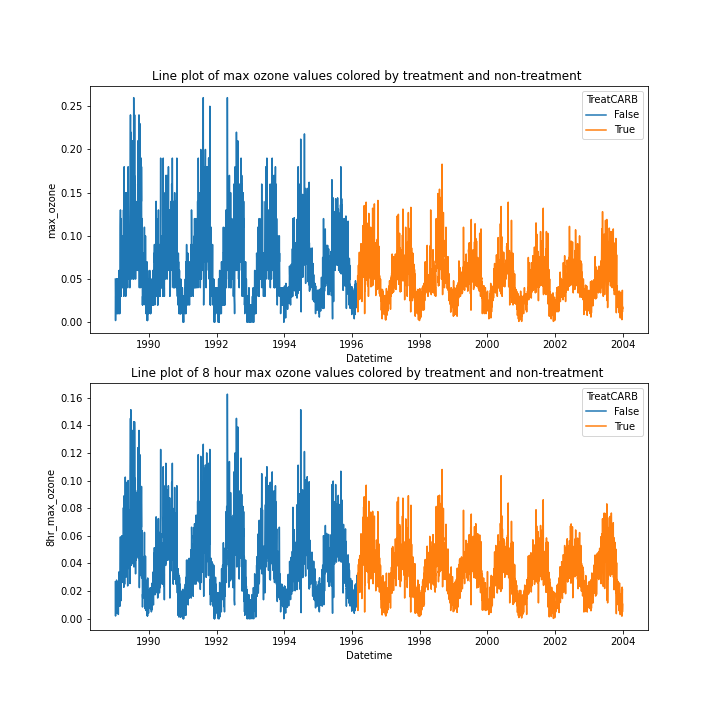
\includegraphics[width=1\textwidth]{all_plot.png}}

\caption{\label{fig:max_all1}Daily ozone measurements over the entire 13 years for Site 1601 in Los Angeles County, California.}
\end{figure}



\begin{figure}[h]
\makebox[\textwidth][c]{
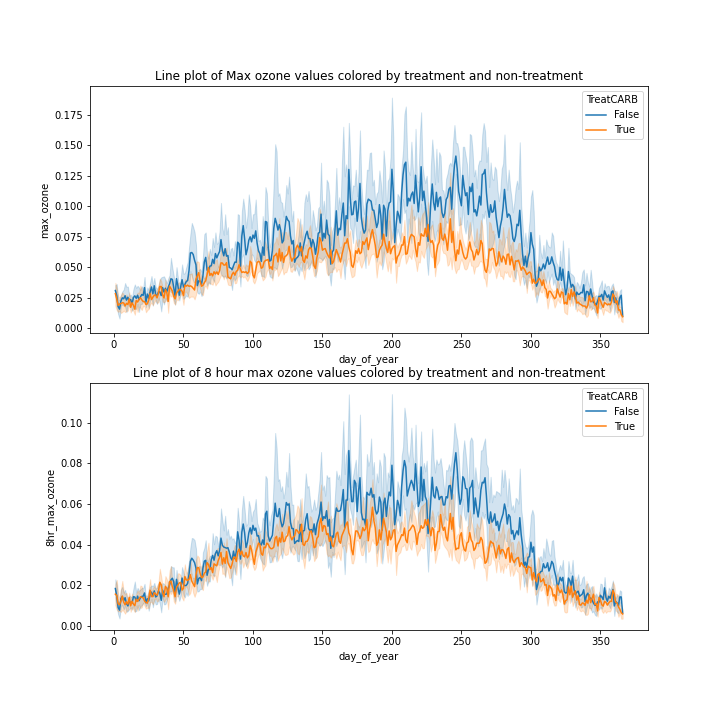
\includegraphics[width=1\textwidth]{day_of_year_ozone.png}}

\caption{\label{fig:max_doy1}Daily ozone measurements before and after CARB was implemented.}
\end{figure}




\begin{figure}[h]
\makebox[\textwidth][c]{
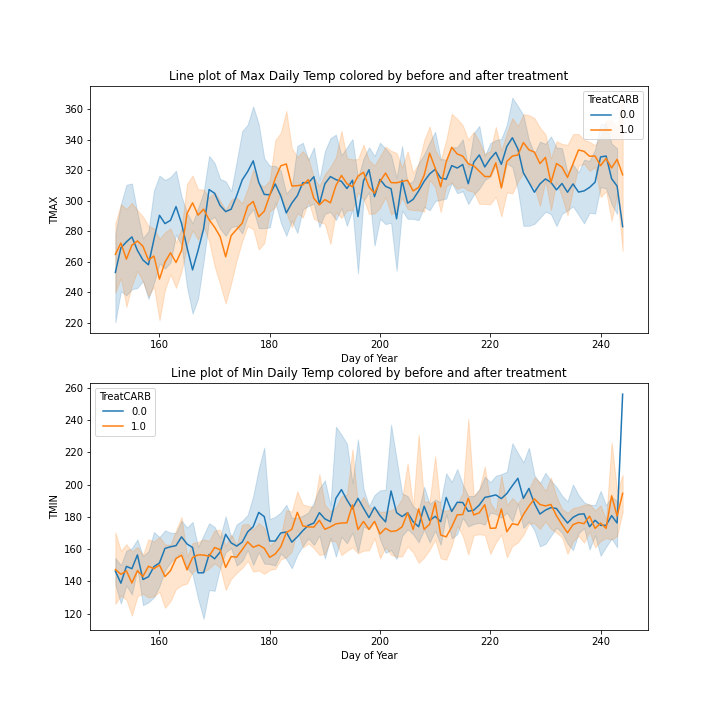
\includegraphics[width=1\textwidth]{control_day_of_yeara.png}}

\caption{\label{fig:control_doyA1}Min and Max temperature over the summer before and after CARB was implemented.}
\end{figure}

\begin{figure}[h]
\makebox[\textwidth][c]{
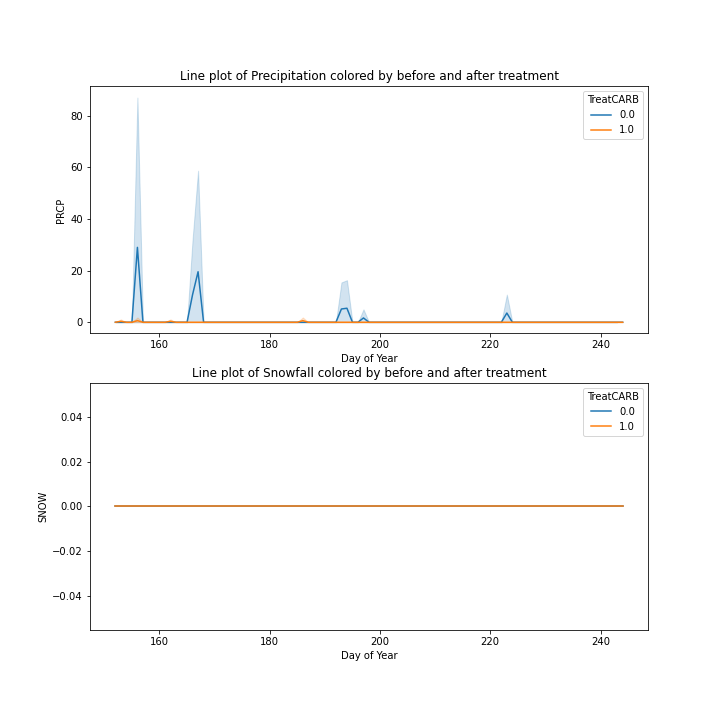
\includegraphics[width=1\textwidth]{control_day_of_yearb.png}}

\caption{\label{fig:control_doyB1}Precipitation and Snowfall over the summer before and after CARB was implemented.}
\end{figure}

\begin{figure}[h]
\makebox[\textwidth][c]{
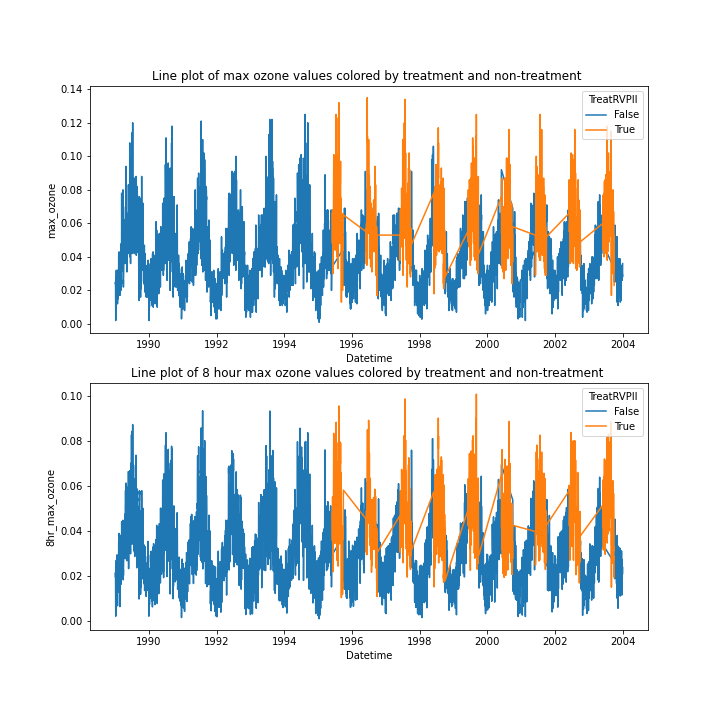
\includegraphics[width=1\textwidth]{all_plot2.png}}

\caption{\label{fig:max_all2}Daily ozone measurements over the entire 13 years for Site 3007 in Madison County, Illinois.}
\end{figure}



\begin{figure}[h]
\makebox[\textwidth][c]{
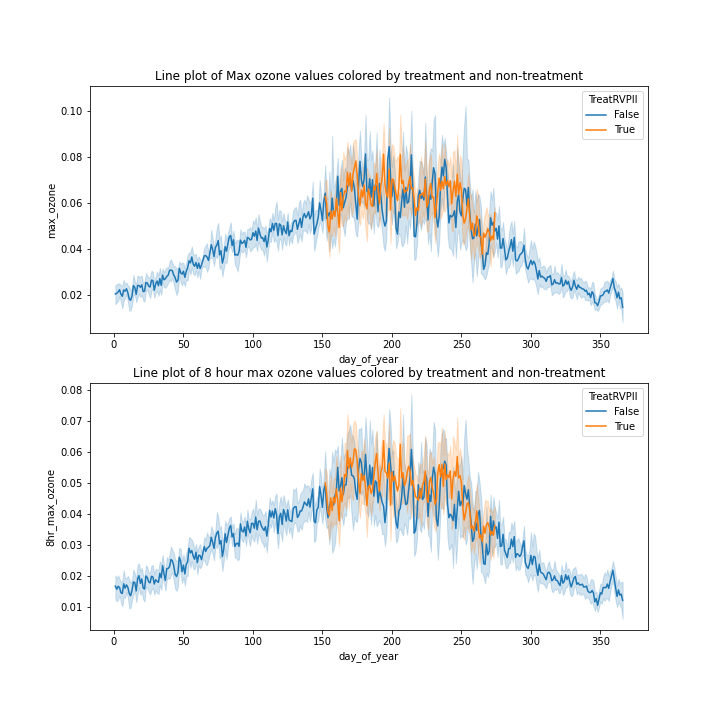
\includegraphics[width=1\textwidth]{day_of_year_ozone2.png}}

\caption{\label{fig:max_doy2}Daily ozone measurements before and after RVPII was implemented.}
\end{figure}




\begin{figure}[h]
\makebox[\textwidth][c]{
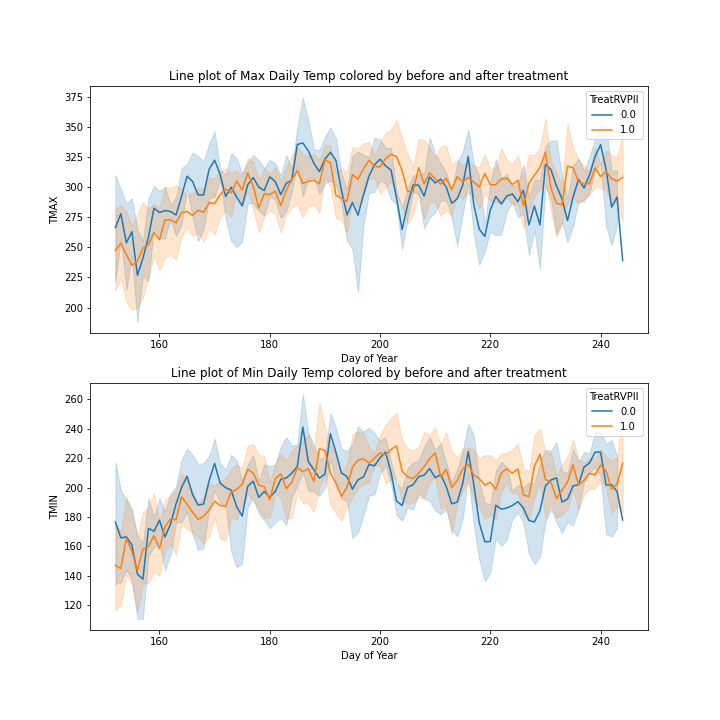
\includegraphics[width=1\textwidth]{control_day_of_year2a.png}}

\caption{\label{fig:control_doyA2}Min and Max temperature over the summer before and after RVPII was implemented.}
\end{figure}

\begin{figure}[h]
\makebox[\textwidth][c]{
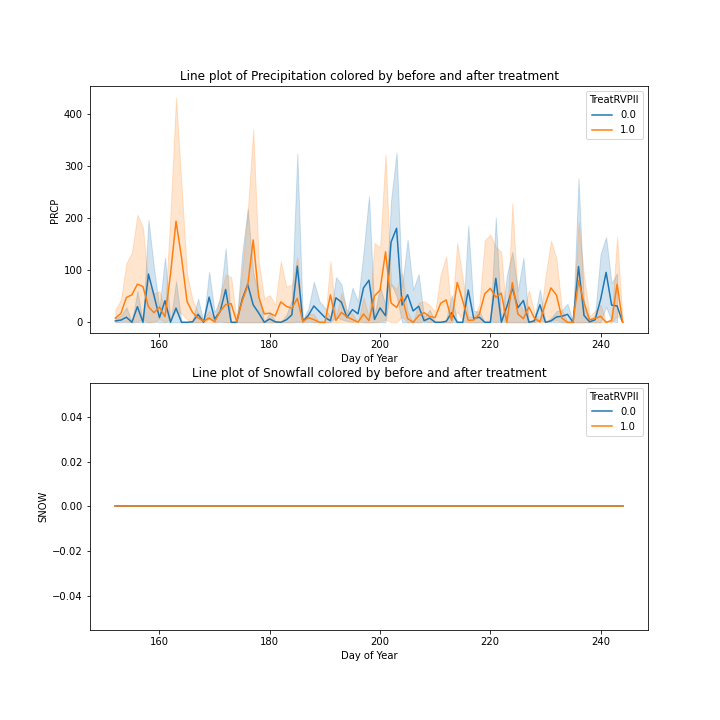
\includegraphics[width=1\textwidth]{control_day_of_year2b.png}}

\caption{\label{fig:control_doyB2}Precipitation and Snowfall over the summer before and after RVPII was implemented.}
\end{figure}


\begin{figure}[h]
\makebox[\textwidth][c]{
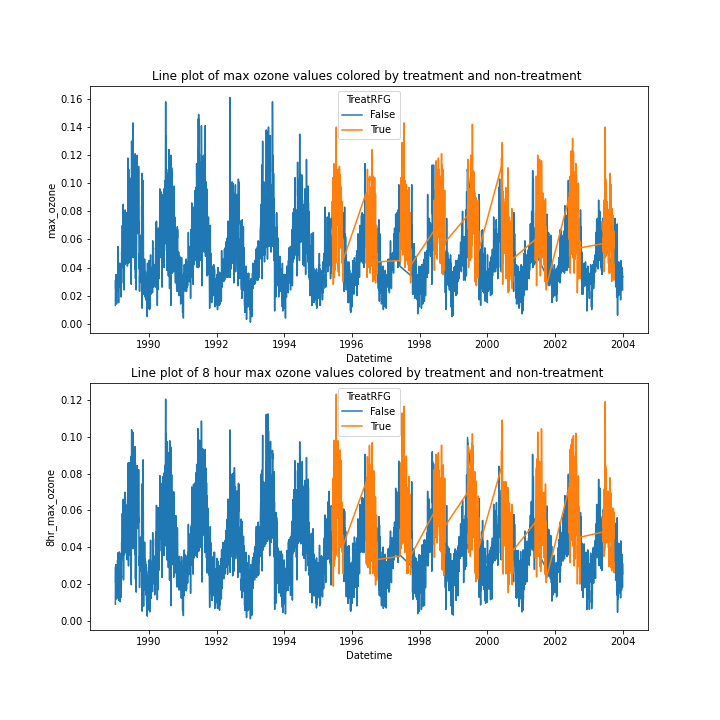
\includegraphics[width=1\textwidth]{all_plot3.png}}

\caption{\label{fig:max_all3}Daily ozone measurements over the entire 13 years for Site 1001 in Cambden County, New Jersey.}
\end{figure}



\begin{figure}[h]
\makebox[\textwidth][c]{
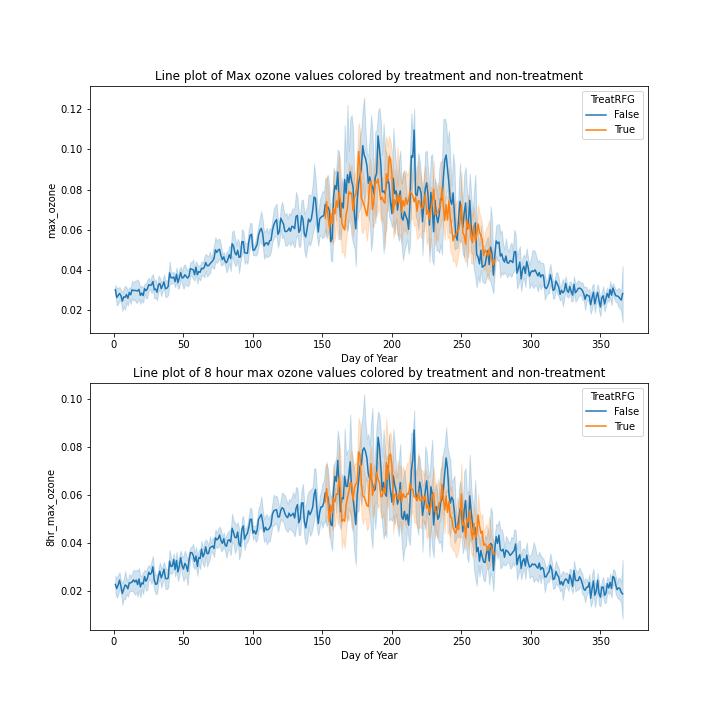
\includegraphics[width=1\textwidth]{day_of_year_ozone3.png}}

\caption{\label{fig:max_doy3}Daily ozone measurements before and after RFG was implemented.}
\end{figure}




\begin{figure}[h]
\makebox[\textwidth][c]{
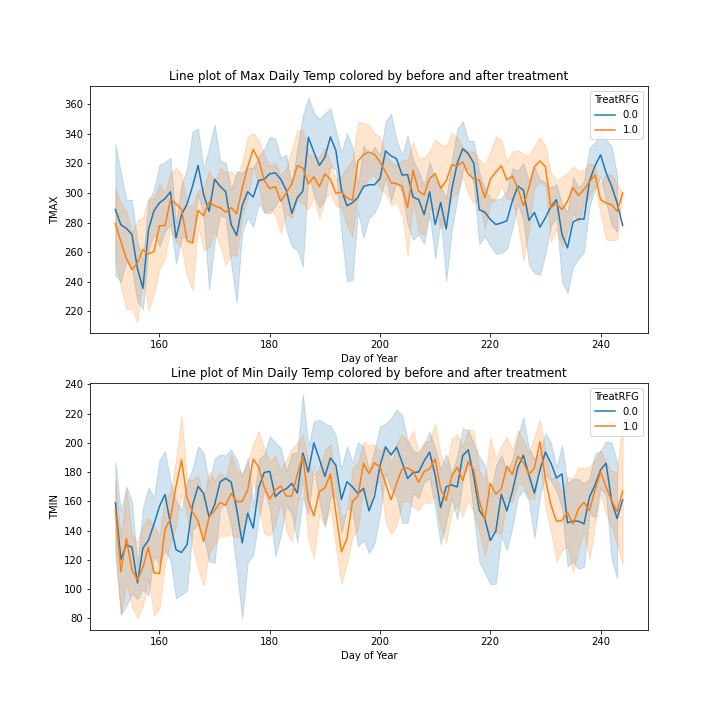
\includegraphics[width=1\textwidth]{control_day_of_year3a.png}}

\caption{\label{fig:control_doyA3}Min and Max temperature over the summer before and after RFG was implemented.}
\end{figure}

\begin{figure}[h]
\makebox[\textwidth][c]{
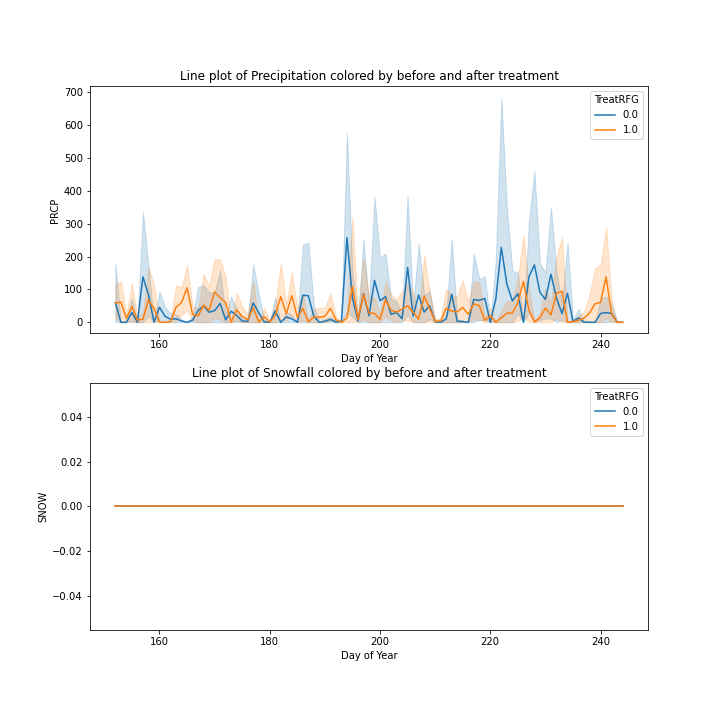
\includegraphics[width=1\textwidth]{control_day_of_year3b.png}}

\caption{\label{fig:control_doyB3}Precipitation and Snowfall over the summer before and after RFG was implemented.}
\end{figure}




\end{document}
